

\textbf{\Large Схема экспериментальной установки}

Схема используемого в работе осмометра приведена на рисунке:

\begin{figure}[H]
	\centering
	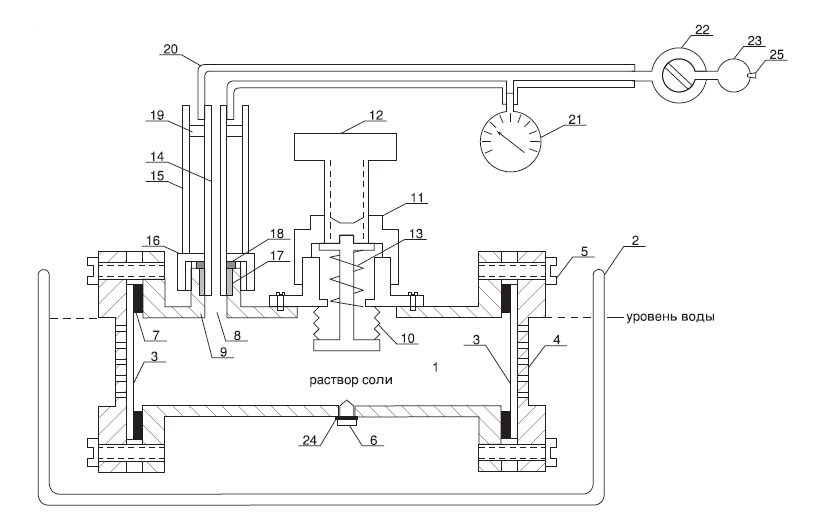
\includegraphics[width=1 \textwidth]{../images/scheme_experiment.png}
\end{figure}

\begin{multicols}{2}
	\begin{spacing}{0.3}
		\begin{enumerate}
			\item Контейнер для раствора соли.
			\item Сосуд с дистиллированной водой.
			\item Целлофановая плёнка.
			\item Защитная сетка.
			\item Прижимной винт.
			\item Пробка-отверстие для заполнения сосуда раствором;
			\item Резиновая прокладка.
			\item Отверстие, через которое раствор поступает в капилляр.
			\item Металлическая втулка, запрессованная в корпус контейнера.
			\item Гофрированная поверхность.
			\item Накидная гайка для грубой регулировки объёма сосуда.
			\item Винт тонкой регулировки объёма.
			\item Пружина.
			\item Стеклянный капилляр.
			\item Металлический кожух капилляра.
			\item Накидная гайка кожуха.
			\item Резиновая трубка, герметизирующая прокладка.
			\item Металлическая шайба.
			\item Подвижная резиновая втулка для крепления капилляра.
			\item Резиновый шланг.
			\item Манометр.
			\item Стеклянный кран.
			\item Резиновая груша для создания повышенного внешнего давления.
			\item Клапан.
		\end{enumerate}
	\end{spacing}

\end{multicols}
	
\newpage
	
Раствор заливается в контейнер 1, который помещается в сосуд с растворителем 2. Контейнер представляет собой куб, закрытый с четырёх сторон полупроницаемыми целлофановыми мембранами 3 толщиной $0,2$ мм. Мембраны зажимаются между стенками куба и металлическими сетками 4, которые предохраняют мембраны от раздувания наружу. Между мембранами и стенками вставлены резиновые уплотнения 7. Сосуд заполняется раствором через отверстие в дне куба, плотно закрываемое металлической гайкой 6 с резиновой прокладкой 21. Через крышку куба вставлен стеклянный капилляр 14, внутренний диаметр $0,5$ мм.

В процессе осмоса объём раствора увеличивается, и уровень раствора движется по капилляру вверх. Скорость подъёма уменьшается при избыточном давлении воздуха на верхнем конце капилляра. Избыточное давление создаётся с помощью груши 23 со встроенный клапаном 25 и фиксируется краном 22. Давление измеряется манометром 21. Кран 22 также позволяет сбросить избыточное давление.

На крышке куба смонтировано устройство, состоящее из гофра 10, накидной гайки 11, винта 12 и пружины 13, позволяющие менять объём внутреннего пространства в кубе. Это бывает необходимо, если в процессе опыта мембраны вытягиваются и уровень раствора в капилляре понижается. При закручивании винта 12 объём контейнера уменьшается и раствор вытесняется в капилляр. Таким образом, уровень раствора можно установить на удобной для наблюдения высоте.



